\begin{tikzpicture}[scale=1.2]
    % draw axes
    \draw (-3,0) to (3,0) node[anchor=north]{$r$};
    \draw[fill] (-1,0)circle(0.5pt) node[anchor=south]{$Q$};

    \draw[fill] (1,0)circle(0.5pt) node[anchor=north west]{$P_{r}$};
    \draw[fill] (1,2)circle(0.5pt) node[anchor=west]{$P$};
    \draw[->] (-1,0) -- (0,0) node[anchor=north]{$\overset{\to}{v_r}$};
    \draw[->] (1,0) -- (1,2);
    \draw(1,1) node[anchor=west]{$d(P,r)$};
    \draw[->] (-1,0) -- (1,2);
    \draw(0,1.5) node{$\overset{\to}{PQ}$};
    %\path[clip] (0,2) -- (0,0) -- (-3,4);
    \fill[color=green!30!black] (-0.5,0) arc (0:45:0.5cm) node[anchor=west]{$\alpha$};
    \fill[color=green!30!black] (-1,0) -- (-0.5,0) -- (-0.635,0.35) -- cycle;
\end{tikzpicture}